\textit{Portions of this chapter were originally published in collaboration with Jake VanderPlas in the September 2018 edition of the Journal of Open Source Software (Fleming and VanderPlas 2018, JOSS, Vol. 3, 29, p. 781; 2018, DOI: 10.21105/joss.00781), and are reproduced below with permission of the Journal of Open Source Software. Portions of this chapter were originally published in collaboration with Rory Barnes, Rodrigo Luger, and Jacob VanderPlas in 2020 in the Astrophysical Journal (Fleming et al. 2020, ApJ, accepted, \textcopyright \ American Astronomical Society), and are reproduced below with permission of the American Astronomical Society.}

In this thesis, I have developed and contributed to numerous theoretical models, all implemented in \vplanet, that simulate the long-term evolution of stars and their planets. In this Chapter, I explore how I can use those models to infer the evolutionary history of exoplanetary systems, in conjunction with observational constraints, using Bayesian statistics. I explain the significant numerical challenges that can make such studies intractible, motivating the development of a software package for rapid, approximate Bayesian inference, \approxposterior. I then describe the \approxposterior algorithm in detail and conclude by discussing in-progress and future work with \approxposterior. 

\section{Introduction: Bayesian Inference with Computationally-Expensive Models}

In order to constrain evolutionary histories of stellar and/or exoplanetary systems using \vplanet, I must calibrate the initial conditions such that the simulation output agrees with the observations, given the observational uncertainties.  This task is mathematically codified by Bayesian inference. Generally, Bayesian inference proceeds as follows:  One seeks to derive a probability distribution for model parameters, e.g. \vplanet initial conditions, given observed data. This distribution is typically referred to as the ``posterior probability distribution". To compute the posterior distribution of a model parameter, \textbf{x}, given observed data, $D$, one uses Bayes' Theorem: $P(\textbf{x} | D) \propto P(D | \textbf{x}) P(\textbf{x})$, where $P(\textbf{x} | D)$ is the posterior probability of \textbf{x} given $D$, $P(\textbf{x})$ is the prior probability assigned to \textbf{x}, and $P(D | \textbf{x})$ is the probability of the data given \textbf{x}, commonly referred to as the likelihood of $D$ given \textbf{x}. This equation neglects the normalization constant, $1/P(D)$, as this is typically quite difficult to compute as it requires integrating the likelihood over the prior. Note that in practice, the natural logarithm of Bayes' Theorem is used. In this case, $\ln P(\textbf{x} | D)$ is known as the ``lnprobability" as it is the natural logarithm of the posterior probability, up to a normalization constant. Note that in this work, I refer to the lnprobabilbiity as $f(\textbf{x})$ for notational connivence. 

For my science applications, I compute the likelihood by running the forward model, \vplanet, to compute a prediction, e.g. a planet's orbital period after Gyrs of tidal evolution, and compare it to the observed values and associated errors, typically using a $\chi^2$ statistic if the uncertainties are assumed to be Gaussian and uncorrelated. Since computing the likelihood requires running a \vplanet simulation and I cannot compute $P(D)$, I must use a Monte Carlo sampling technique to estimate the posterior distribution. This procedure is usually done using Markov Chain Monte Carlo (MCMC) methods, such as the affine-invariant MCMC code, \emcee, that is commonly used in astronomy \citep{ForemanMackey2013}. Standard MCMC runs, however, can require upwards of $10^6$ likelihood calculations, depending on the dimensionality of the problem, to draw a suitable number of samples from the posterior distribution and build up statistical power.  In this case, a simple \vplanet simulation of the stellar and tidal evolution of an exoplanetary system, which takes one minute to run, would require about 2 years of core-hours for a single MCMC run, rendering this technique computationally intractable at scale. Clearly, for Bayesian inference to become feasible for slow models, a method to compute the posterior distribution while minimizing the number of forward model evaluations is required. 

I address this issue and enable Bayesian parameter inference with \vplanet by developing \approxposterior, an open-source Python implementation of the ``Bayesian Active Posterior Estimate" (BAPE) algorithm created by \citet{Kandasamy2017}.

\section{Fast and Accurate Approximate Bayesian Inference with \approxposterior}

\approxposterior is a Python package for efficient approximate Bayesian inference and Bayesian optimization of computationally-expensive models. \approxposterior implements both the Bayesian Active Learning for Posterior Estimation (BAPE, \citet{Kandasamy2017}) and Adaptive Gaussian process approximation for Bayesian inference with expensive likelihood functions (AGP, \citet{Wang2018}) algorithms. \approxposterior generalizes these algorithms by including several modifications to improve the accuracy and afford the user more control over the inference. In practice \approxposterior uses machine learning by training a Gaussian process \citep[GP][]{Rasmussen2006} surrogate, or emulator, for the computationally-expensive model. That is, the GP learns to predict the lnprobability uses in Bayes' Theorem, $f(\textbf{x})$, such that the trained GP is used with an MCMC sampling method to obtain the posterior probability distribution for the forward model parameters. 

Crucially, \approxposterior employs an active learning approach to iteratively improve the GP's predictive performance while minimizing the number of calls to the expensive model required to generate the GP's training set, significantly reducing the computational cost. Both algorithms implemented by \approxposterior, BAPE and AGP, include a similar active learning approach to intelligently expand the GP training set, so I will just describe the BAPE formalism for brevity. BAPE and AGP both leverage the fact that each evaluation of the GP conditional predictive distribution, or each GP prediction of $f(\textbf{x})$, is a one-dimensional Gaussian distribution.  BAPE actively identifies high-likelihood, and hence high posterior probability, regions in parameter space where the GP predictions are uncertain, i.e. a wide Gaussian distribution at that point.  The algorithm then runs the forward model in these regions to supplement its training set, maximizing the improvement of the GP's predictive ability.  The GP then becomes an accurate surrogate for the forward model by training on few evaluations in regions of parameter space that are relevant to the inference, minimizing the computational cost to estimate posterior probability distributions for model parameters. 

Below, I qualitatively describe the \approxposterior algorithm, define its parameters, and suggest typical values. 

\section{\approxposterior Algorithm} \label{AP:sec:app}

Qualitatively, the \approxposterior algorithm is as follows. First, assume a forward model with $d$ input parameters that is designed to reproduce some set of observations. In our case, $d$, the dimensionality of parameter space, is five. The model parameters have an input domain, $D$, that is defined by the user. The parameters are further described by a prior probability distribution based on the user's prior belief for how the model parameters are distributed.  Next, the user generates a training set, $T$, consisting of $m_0$ forward model simulations distributed across the parameter space. The user chooses how the $m_0$ samples are distributed throughout parameter space according to their preferred experimental design. \approxposterior then trains a GP on $T$ to construct a non-parametric model (sometimes called a ``surrogate model") that represents the outcomes of the forward model over the parameter space. Crucially, GPs also generate an uncertainty for the surrogate model at every point in parameter space.

\approxposterior then identifies $m$ more locations in parameter space to apply the forward model and add to $T$. The new locations are selected by determining the regions that the GP has identified as having both a high lnprobability, i.e. high posterior density, and a high predictive uncertainty. This selection is accomplished by maximizing a utility function ($u$, described below) that quantifies where the GP predicts high posterior density and high uncertainty in parameter space, focusing resources on parameter combinations that are likely to be consistent with the observations. \approxposterior re-trains the GP with the augmented $T$. The GP is then passed to an MCMC algorithm, e.g. \emcee, that samples the parameter space to obtain the approximate posterior distributions of the model parameters.

At the end of each iteration, \approxposterior checks if a convergence condition (described in $\S$~\ref{AP:sec:app:convergence}) has been met. If the algorithm  has not yet converged, \approxposterior selects an additional $m$ new points to add to $T$, re-trains the GP, and again estimates the posterior distribution. This process repeats until convergence or until \approxposterior has run the maximum number of iterations, $n_{max}$, set by the user. In Algorithm~\ref{AP:app:algo}, we list the aforementioned steps that comprise this algorithm.

\begin{algorithm} 
\SetAlgoLined
 Assume an input domain $D$, GP prior on $f(\textbf{x})$ \\
 Generate a training set, $T$, consisting of $m_0$ pairs of $(\textbf{x}, f(\textbf{x}))$ \\
 \For{$t=0, 1, ..., n_{\mathrm{max}}$}{
    \For{$i=0, 1, ..., m$}{
      Find \textbf{x}$^+$ = argmax$_{\textbf{x} \in D}$ $u(\textbf{x})$ \\
       Compute $f(\textbf{x$^+$})$ \\
       Append $(\textbf{x$^+$}, f(\textbf{x$^+$}))$ to $T$ \\
       Re-train GP, optimize GP hyperparameters given augmented $T$ \\
   }
   Use MCMC to obtain approximate posterior distribution with GP surrogate for $f(\textbf{x})$ \\
   \If{$\mathrm{converged}$}{
        \textbf{break} \\
    }
 }
\caption{\approxposterior Approximate Inference Pseudo Code  \label{AP:app:algo}}
\end{algorithm}
where $f(\textbf{x}) = \mathcal{\ln L}(\textbf{x})$ + $\ln \mathrm{Prior}(\textbf{x})$, i.e. the lnprobability function used for MCMC sampling with \emcee and \textbf{x}$^+$ is the point in parameter space selected by maximizing $u$. For our application, evaluating $f(\textbf{x})$ requires running a \vplanet simulation to compute $\mathcal{\ln L}(\textbf{x})$ (see $\S$~\ref{trap:sec:mcmc:like}).

By placing a GP prior with a squared exponential kernel on $f(\textbf{x})$, we assume that the function is smooth and continuous, both reasonable assumptions for modeling the posterior density. For inference problems that are liable to violate these assumptions, other kernels, e.g. the Ornstein-Uhlenbeck kernel, may be more appropriate (we refer the reader to \citet{Rasmussen2006} for detailed descriptions of common GP kernels and their mathematical properties). \approxposterior uses \texttt{george} \citep{george} for all GP calculations and hence users can apply any kernels implemented in that software package.

\approxposterior has several free parameters that can be set by the user: $m_0$, the size of the initial training set (50 in our case), $n_{\mathrm{max}}$, the maximum number of iterations (15), $m$, the number of new points to select each iteration where the forward model will be evaluated (50 per iteration), and $\epsilon$, the convergence threshold (0.1). Typically, we find that $n_{\mathrm{max}}=2-3 \times d$, $m, m_0 = 10-20 \times d$, and $\epsilon = 0.1$ work well in practice, although performance may vary depending on the use case. For a complete list of \approxposterior parameters, we refer the reader to the online documentation.\footnote{ \href{https://dflemin3.github.io/approxposterior}{https://dflemin3.github.io/approxposterior/}}

Note that \approxposterior does not linearly transform the parameter space to the unit hypercube as did \citet{Kandasamy2017}. Moreover, \approxposterior does not fix the covariance scale lengths, instead opting to estimate all GP kernel hyperparameters by maximizing the marginal likelihood of the GP, given its training set, at a user-specified cadence. In Algorithm~\ref{AP:app:algo}, we optimize the GP hyperparameters each time a new point is added to the training set, but in practice we found this is unnecessary, especially at later iterations when the GP has developed a reasonable approximation of the posterior. The authors prefer to optimize the GP hyperparameters twice per iteration, once after half of the $m$ new points have been selected, and again after all $m$ points have been selected.

\section{\approxposterior: Theory and Practical Usage} \label{ap:sec:usage}

In this section, I further describe \approxposterior's training set augmentation procedure and how to check for convergence in $\S$~\ref{AP:sec:augment} and $\S$~\ref{AP:sec:app:convergence}, respectively. I examine how the \approxposterior training set augmentation and convergence procedures work in practice for the science case explored in Chapter 6.  I then provide a simple example of an \approxposterior Python script that reproduces the \citet{Wang2018} test to both validate \approxposterior and show its practical usage in $\S$~\ref{AP:sec:example}. Finally in $\S$~\ref{AP:sec:docs}, I comment on \approxposterior's extensive online examples and documentation.

\subsection{Augmenting the Training Set} \label{AP:sec:augment}

Each iteration, \approxposterior selects $m$ new points to add to the GP's training set by maximizing the utility function, $u$. To motivate the choice of $u$, consider the following argument based on \citet{Kandasamy2017}: \approxposterior assumes that the forward model the GP learns on, here \vplanet via $\ln \mathcal{L}$, is computationally-expensive to run, and hence \approxposterior seeks to minimize the number of forward model evaluations required to build its training set. For inference problems, it is natural to select high-lnprobability regions in parameter space to augment the GP training set as this is where the posterior density is large. Furthermore, selecting regions in parameter space where the GP's predictive uncertainty is already small offers little value, compared to regions where its predictions are more uncertain, as additional points in low-uncertainty regions are unlikely to alter the GP's predictions. 

With these considerations in mind, \citet{Kandasamy2017} leverage the analytic properties of GPs to derive the ``exponentiated variance" utility function, given by their Eqn.~(5)
\begin{equation} \label{AP:eq:bape}
    u_{\textrm{EV}}(\textbf{x}) = \exp(2 \mu_t(\textbf{x}) + \sigma_t^2(\textbf{x}))(\exp(\sigma_t^2(\textbf{x})) - 1),
\end{equation}
where $\mu_t(\textbf{x})$ and $\sigma_t^2(\textbf{x})$ are the mean and variance of the GP's predictive conditional distribution evaluated at \textbf{x}, respectively, for the $t^{th}$ \approxposterior iteration. Using the same parameters, \citet{Wang2018} derive a similar entropy-based utility function given by their Eqn.~(7)
\begin{equation} \label{AP:eq:agp}
    u_{\textrm{AGP}}(\textbf{x}) =\mu_t(\textbf{x}) + \frac{1}{2} \ln(2 \pi e \sigma_t^2(\textbf{x})).
\end{equation}
\approxposterior defaults to using Eqn.~\ref{AP:eq:bape}. Therefore to select each point, \approxposterior maximizes Eqn.~\ref{AP:eq:bape} using the Nelder-Mead method \citep{Nelder1965}. Note that this optimization is rather cheap since it only requires evaluating the GP's predictive conditional distribution, so this task is not a significant computational bottleneck. I restart this optimization 5 times to reduce the influence of local extrema. Note that in practice, I optimize the natural logarithm of the utility function to ensure numerical stability.

\begin{figure}
	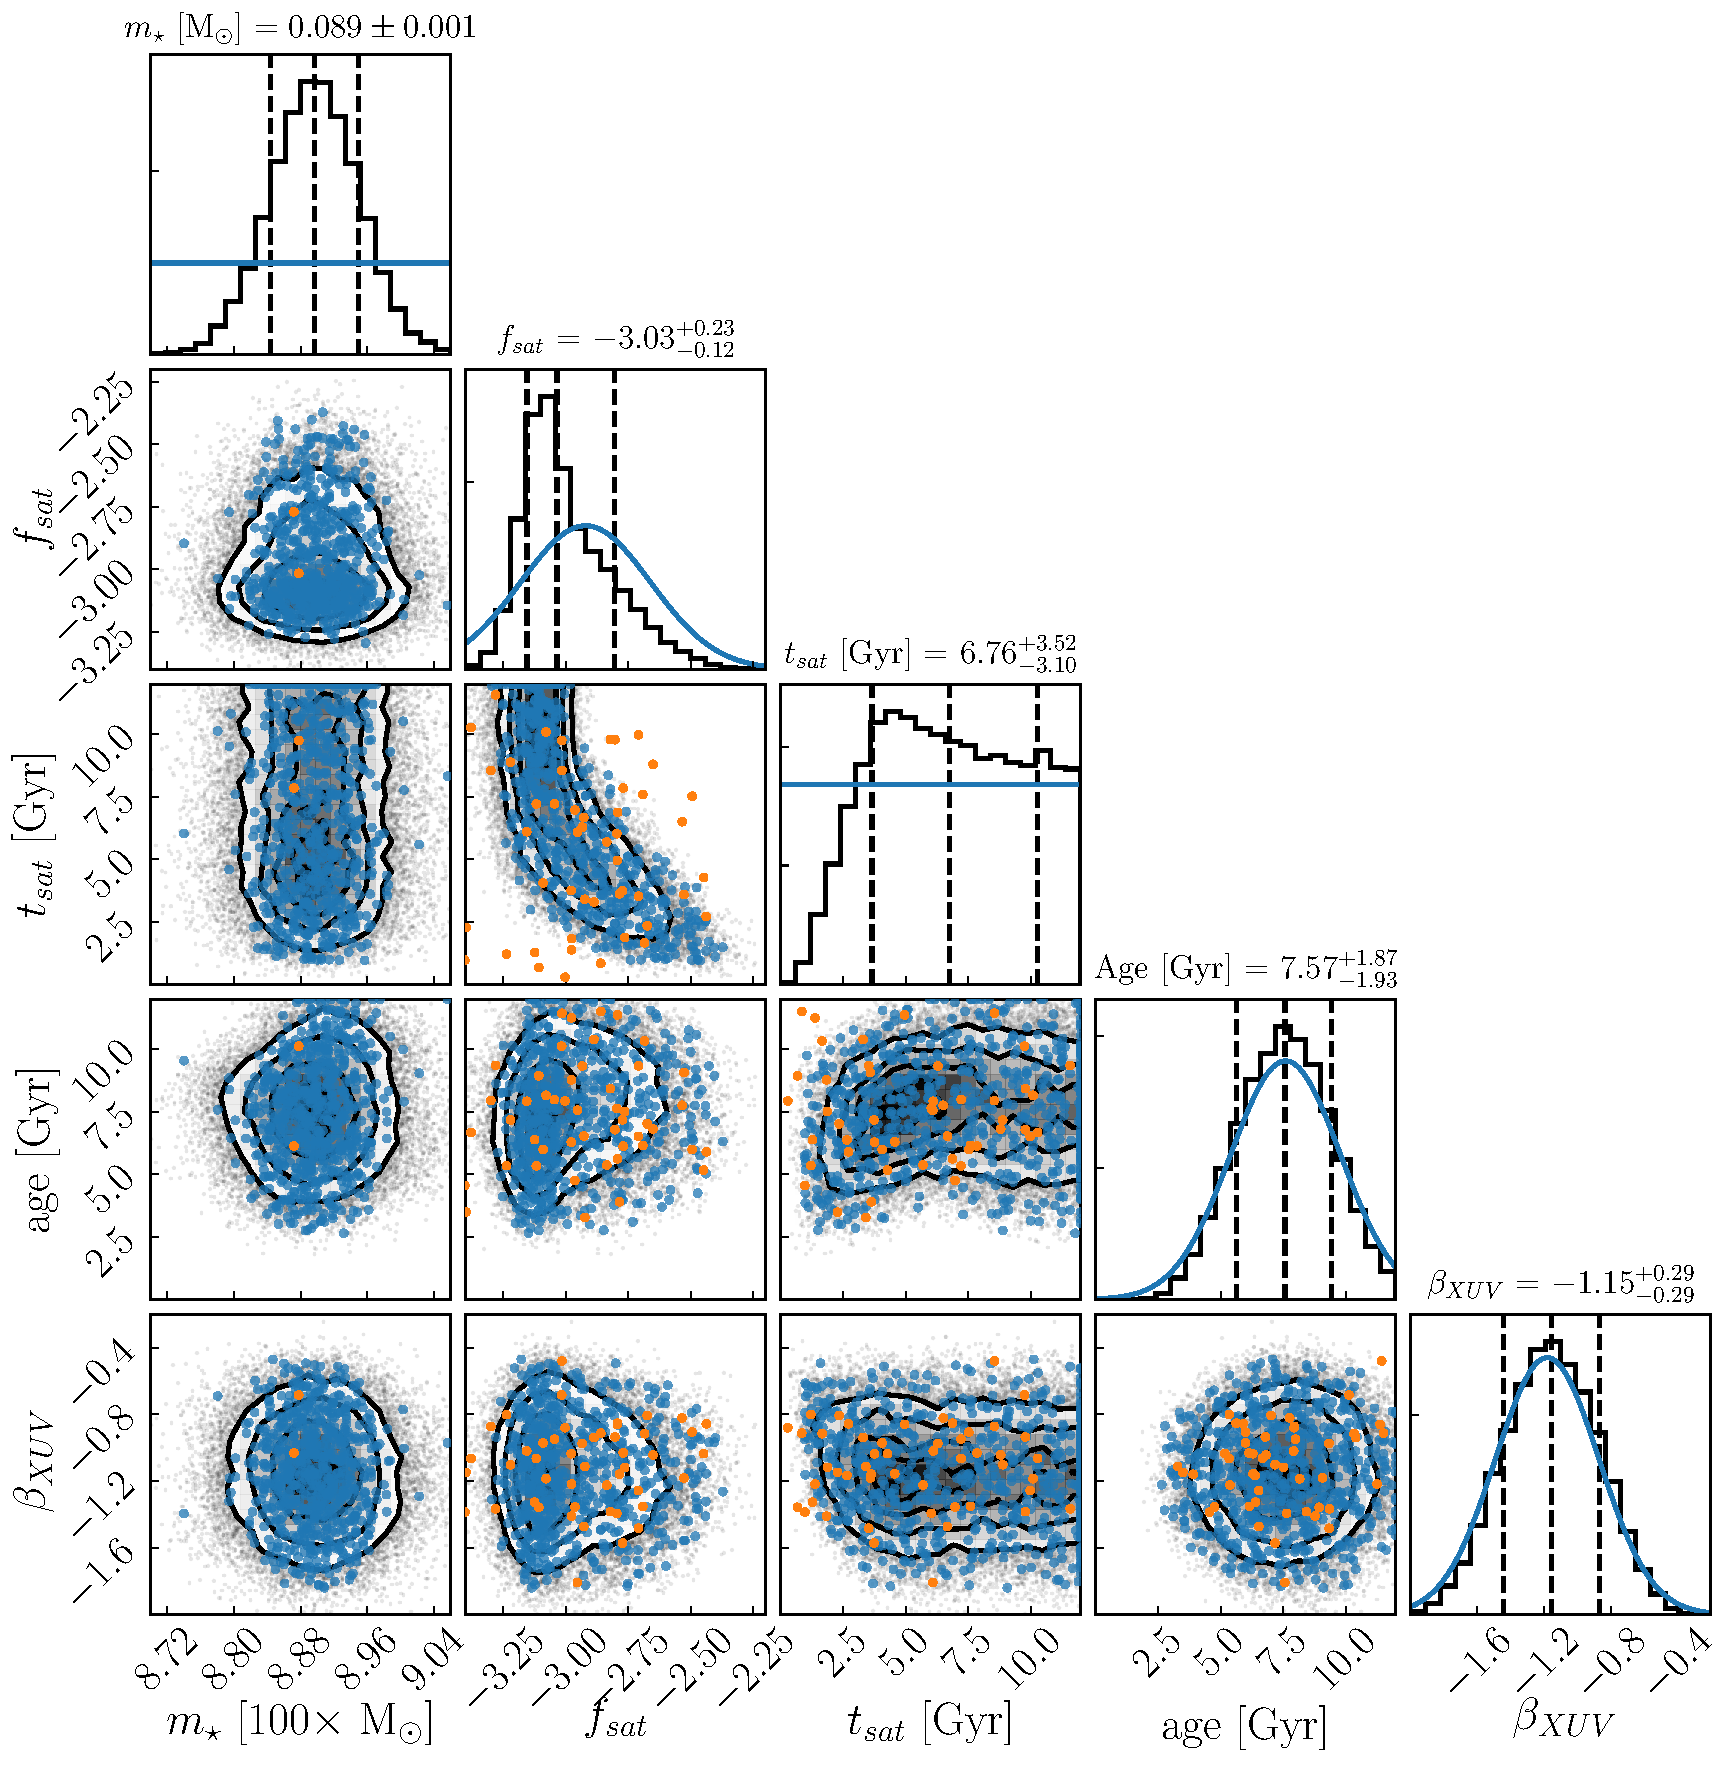
\includegraphics[width=\textwidth]{points.pdf}
   \caption{Same as Fig.~\ref{trap:fig:approx}, but overplotted with the training set for \approxposterior's GP. The orange points display the initial training points whereas the blue points display the points iteratively selected by maximizing the \citet{Kandasamy2017} utility function, Eqn.~(\ref{AP:eq:bape}). By design, \approxposterior selected points to expand its training set in regions of high posterior density, improving its GP's predictive accuracy in the most relevant regions of parameter space while seldom wasting computational resources in the low likelihood regions.}%
    \label{AP:fig:points}%
\end{figure}

As demonstrated in \citet{Kandasamy2017}, Eqn.~(\ref{AP:eq:bape}) identifies high-likelihood points where the GP's predictions are uncertain, significantly reducing the cost of training an accurate GP surrogate model. We highlight this behavior for our own application in Fig.~\ref{AP:fig:points} by displaying the approximate posterior distribution derived by \approxposterior from \citet{Fleming2020} overplotted with the initial training set in orange and the points selected by sequentially maximizing Eqn.~(\ref{AP:eq:bape}) in blue. Given the small initial training set, \approxposterior successfully selects high-posterior density points in parameter space to augment the GP's training set. Some points are selected in low-likelihood regions early on, typically near the edges of parameter space where the GP's uncertainty was initially large.

% extra
%\xxx{\citet{Wang2018} derive the entropy-based utility function (``Adaptive Gaussian Process", AGP) that is designed to select the point \textbf{x} that, when added to the GP training set $T$, maximizes the information gain for the inference problem. The \citet{Wang2018} utility function given by their Eq.~(7)}
%\begin{equation} \label{app:eq:agp}
%    u_{\textrm{AGP}}(\textbf{x}) = \mu_t(\textbf{x}) + \frac{1}{2}\ln{(2\pi e \sigma_t^2(\textbf{x}))}
%\end{equation}
%where $e$ is Euler's number.

\subsection{Convergence} \label{AP:sec:app:convergence}

We assess the convergence of the \approxposterior algorithm by comparing the means of the approximate marginal posterior distributions over successive iterations. We consider an \approxposterior run ``converged" if the differences between the marginal posterior means, relative to the widths of the marginal posteriors, are less than a tolerance parameter, $\epsilon$, for $k_{max}$ consecutive iterations. Effectively, this criterion checks if the expected value of each model parameter over the posterior distribution varies by ${\leq}{\epsilon}$ standard deviations from the previous iteration's expected values. That is, we require the \approxposterior convergence diagnostic $z_{t,j}{\leq}{\epsilon}$ for all $j$, where
\begin{equation}
    z_{t,j} = |\mu_{t,j} - \mu_{t-1,j}| / \sigma_{t-1,j},
\end{equation}
 and $\mu_{t,j}$ and $\sigma_{t,j}$ are the mean and standard deviation of the approximate marginal posterior distribution for the $t^{th}$ iteration and the $j^{th}$ parameter. This quantity is analogous to the ``z-score" commonly used in many statistical tests. Following \citet{Wang2018}, we require this condition to be satisfied for $k_{max}$ consecutive iterations to ensure \approxposterior is producing a consistent result. With this scheme, \approxposterior tolerates deviations from the previous estimate that are less than, or at least consistent with, the previous values, given the inherent uncertainty implied by the width of the posterior distribution. For our application, we adopted conservative choices of $\epsilon = 0.1$ and $k_{max} = 5$. Each \approxposterior iteration, we also visually inspected the estimated posterior distribution to ensure convergence. 

In Fig.~\ref{AP:fig:convergence}, we display the convergence diagnostic quantity, $z_t$, as a function of iteration for each model parameter for the \approxposterior run presented in the main text. \approxposterior quickly finds a consistent result as $z_t$ decreases below our convergence threshold within the first few iterations. For each parameter, $z_t$ continues to decrease until iteration 3 before stabilizing. The evolution of $z_t$ is not monotonic, however, owing to the stochastic nature of GPs, our hyperparameter optimization scheme, and MCMC sampling that can cause these values to occasionally be slightly worse than previous iterations. Requiring convergence over $k_{max}$ consecutive iterations mitigates the impact of this stochasticity.

\begin{figure}
\centering
	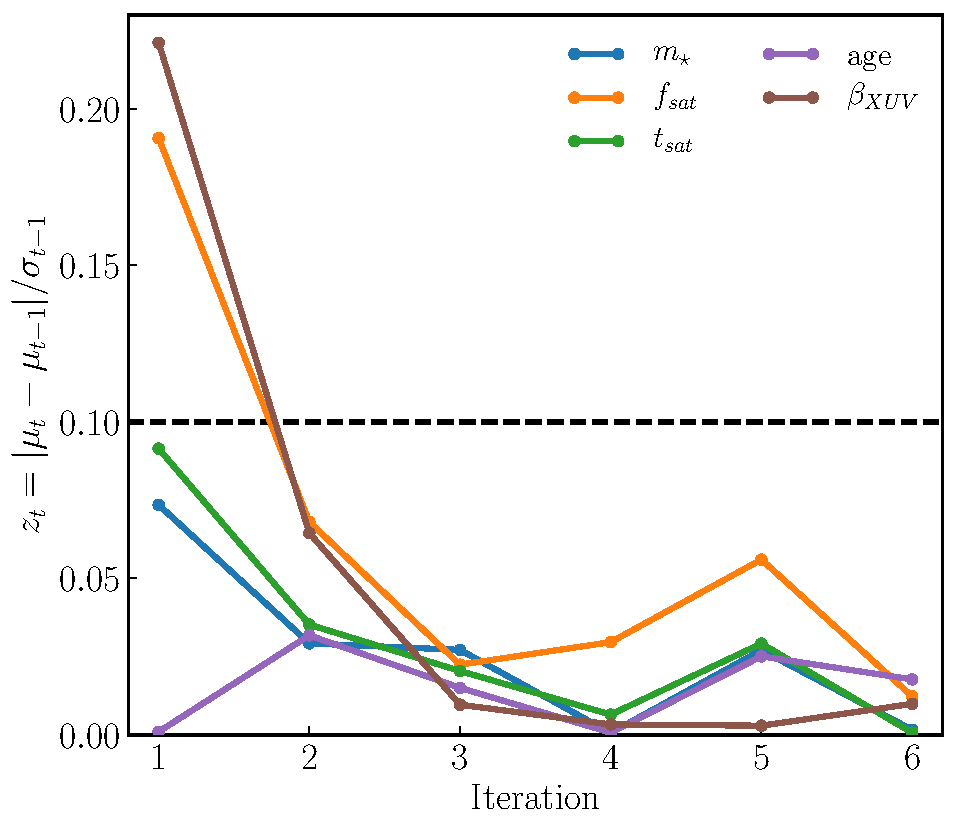
\includegraphics[width=\textwidth]{convergence.pdf}
   \caption{The \approxposterior convergence diagnostic, $z_t$, as a function of iteration for the run presented in the main text. Note that in \approxposterior, the initial iteration is iteration 0. The black dashed line indicates our adopted convergence threshold of $\epsilon = 0.1$. \approxposterior quickly converges to a consistent and accurate result.}%
    \label{AP:fig:convergence}%
\end{figure}

\subsection{A Simple Example} \label{AP:sec:example}
Below, I include a simple Python script for running \approxposterior.\footnote{The full example Python script is publicly available at \href{https://github.com/dflemin3/approxposterior/blob/master/examples/inference/example.py}{https://github.com/dflemin3/approxposterior/blob/master/examples/inference/example.py}}

\inputpython{example.py}{1}{39}

\subsection{Online Documentation} \label{AP:sec:docs}

\approxposterior has extensive online documentation located on both its GitHub page\footnote{\href{https://github.com/dflemin3/approxposterior}{https://github.com/dflemin3/approxposterior}} and on an additional public documentation website.\footnote{\href{https://dflemin3.github.io/approxposterior/}{https://dflemin3.github.io/approxposterior/}} The online examples comprise both annotated Jupyter Lab notebooks and commented Python scripts, like the one shown above, to allow new users understand how \approxposterior is called and used in practice. Moreover, the online documentation includes the full \approxposterior API; each parameter in every \approxposterior class and function is fully described, including what the parameter and reasonable default values. The online documentation serves to help new users employ \approxposterior in their own research. As the primary author of \approxposterior, I encourage new users to both fully read the online documentation and run all examples before developing scripts for their own application.

\section{Future Applications: Terrestrial Exoplanet Atmospheric Retrieval} \label{AP:sec:future}

Finally, I discuss additional an application of \approxposterior to atmospheric retrieval problems to highlight its flexibility and potential for enabling Bayesian inference studies with computationally-expensive models.

The following papers all use various flavors of neural networks for atmospheric retrieval: \citep{Waldmann2016,MarquezNeila2018,Zingales2018,Cobb2019,Fisher2019,Himes2020}.

\begin{figure}
\centering
	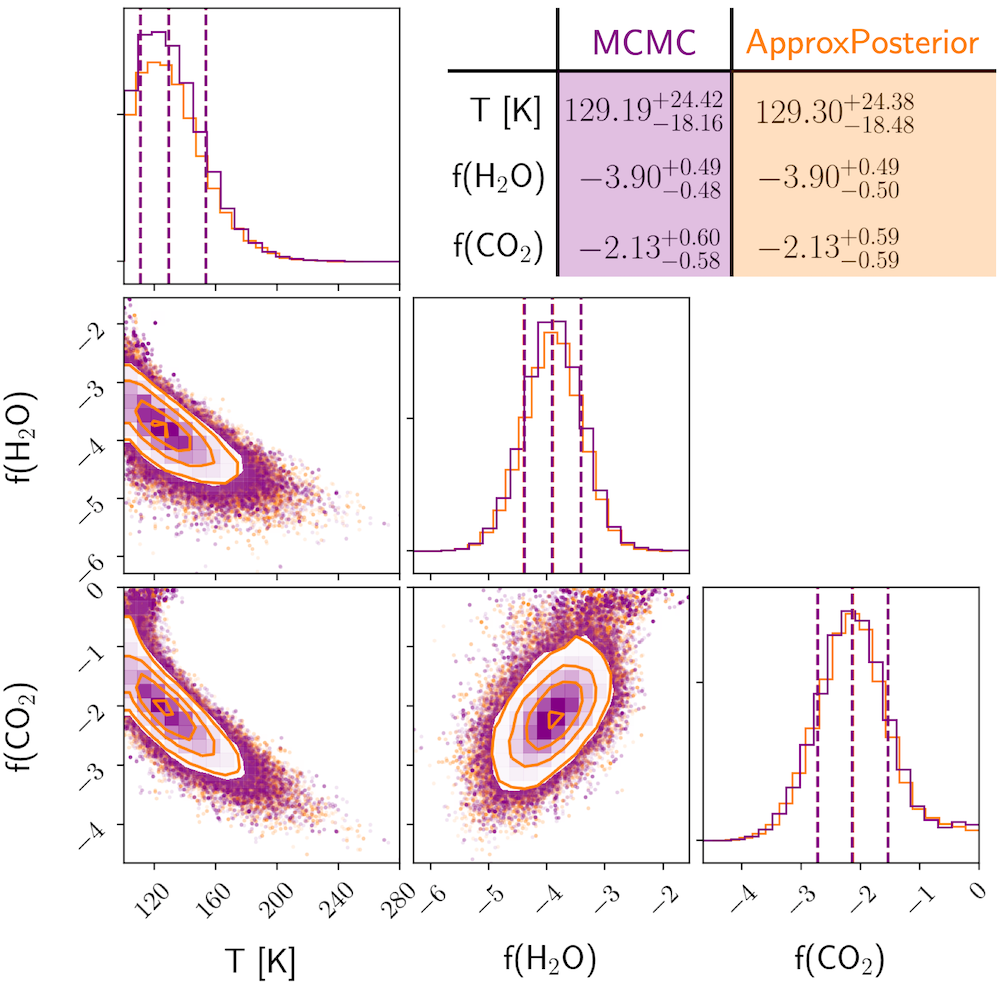
\includegraphics[width=\textwidth]{emceeAPComparison.png}
   \caption{Joint and marginal posterior probability distributions derived by \emcee (purple) and \approxposterior (orange) from an atmospheric retrieval of a simulated noised JWST transmission spectrum of TRAPPIST-1e (used with permission from Lustig-Yaeger et al., in prep). This retrieval experiment attempts to infer the isothermal atmospheric temperature, $T$, and the mixing ratios of H$_2$O and CO$_2$. \approxposterior accurately recovers both the nontrivial correlations between model parameters and marginal parameter constraints as did \emcee, within Monte Carlo error, but requiring about 1000 times fewer computational resources.}%
    \label{AP:fig:comparison}%
\end{figure}


